% ============PREAMBLE SECTION==========================================
%+++++++++++++++++++++++++++++++++++++++++++++++++++++++++++++++++++++++
\documentclass[12pt]{article}
\usepackage{geometry}                % See geometry.pdf to learn the layout options. There are lots.
\geometry{letterpaper}                   % ... or a4paper or a5paper or ... 
%\geometry{landscape}                % Activate for for rotated page geometry
\usepackage[parfill]{parskip}    % Activate to begin paragraphs with an empty line rather than an indent
\usepackage{daves,fancyhdr,natbib,graphicx,dcolumn,amsmath,lastpage,url}
\usepackage{amsmath,amssymb,epstopdf,longtable}
\DeclareGraphicsRule{.tif}{png}{.png}{`convert #1 `dirname #1`/`basename #1 .tif`.png}
\pagestyle{fancy}
\lhead{Student Name: \_\_\_\_\_\_\_\_\_\_\_\_\_\_\_\_\_\_\_\_\_\_\_\_\_\_\_\_\_\_\_\_\_\_\_\_\_\_\_\_\_\_\_\_\_ }
\rhead{FALL 2024}
\lfoot{CE 3354 Engineering Hydrology }
\cfoot{EXAM 2}
\rfoot{Page \thepage\ of \pageref{LastPage}}
\renewcommand\headrulewidth{0pt}

% other
\usepackage{paralist}  % need to modify standard enumerate blocks
%=========Longtable environment
\usepackage{setspace}                % allow single and double space environment
\usepackage{longtable}                % allow table to span multiple pages
\usepackage{caption}                    % consistent caption package
\usepackage{url}					% Ubiquitious url formatting package
%===========

\DeclareGraphicsRule{.tif}{png}{.png}{`convert #1 `dirname #1`/`basename #1 .tif`.png}
%++++++++++++++++++++++++++++++++++++++++++++++++++++++++++++++++++++++++++
%============================================================================
\begin{document}

\begingroup
\begin{centering}
\textbf{CE 3354 Engineering Hydrology} \\
\textbf{Exam 2, Fall 2024}\\
\end{centering}
~\\
Students should write their name on \textbf{all sheets of paper}.  \newline 
Students are permitted to use the internet, their own notes and the textbook.  \newline 
Students are \textbf{forbidden} to \textbf{communicate with other people} during the examination.
\endgroup
%%%%%%%%%%%%%%%%%%%%%%%%%%%%%%%%%%%%%%%%%%%%%%%%%%%%%%
\begin{enumerate}
%%%%%% MULTIPLE GUESS PORTION %%%%%%%%%%%%%%%%%%%%
\item Figure \ref{fig:watercycle} below shows a model of the water cycle. 
The arrows show the movement of water molecules through the water cycle. 
The circled numbers processes that dominate as the water molecules reach the different stages of the water cycle. \newline
\begin{figure}[h!] %  figure placement: here, top, bottom, or page
   \centering
   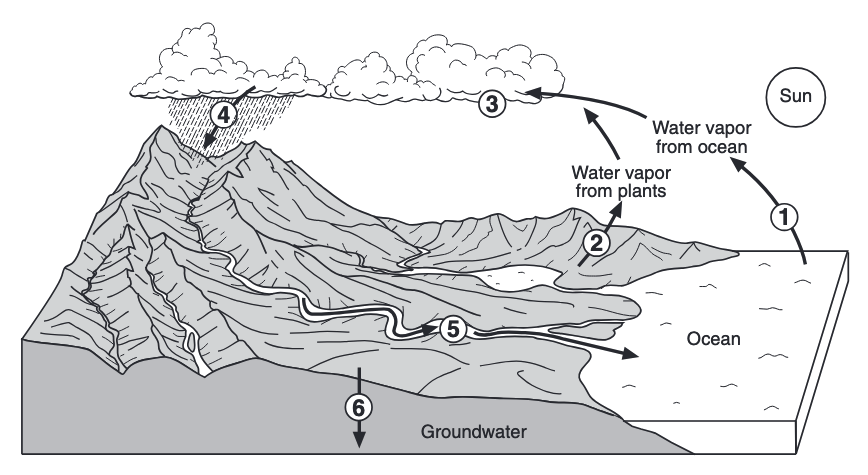
\includegraphics[width=5in]{watercycle.png} 
   \caption{Water Cycle Diagram}
   \label{fig:watercycle}
\end{figure}

Complete Table \ref{tab:watercycle} by the water cycle process occurring at each number.
\begin{table}[h!]
\centering
\caption{Dominant Water Cycle Process}
\begin{tabular}{p{1.0in}p{4in}} % Column formatting, @{} suppresses leading/trailing space
Item &: Water Cycle Process\\
\hline
1 &: ~ \\
\hline
2 &: ~ \\
\hline
3 &: Condensation (into clouds) \\
\hline
4 &: ~ \\
\hline
5 &: ~ \\
\hline
6 &: ~ \\
\hline
\end{tabular}
\label{tab:watercycle}
\end{table}
\clearpage
%%%%%%%%%%%%%%%%%%%%%%%%%%%%%%%%%%%%%%%%%%%%%%%%%%%%
\item Consider the two graphs in Figure \ref{fig:hydrographs}, which show the relationship between the amount of rainfall during a storm and the amount of discharge in a nearby stream. Letter A represents the time when approximately 50\% of the precipitation from the storm has fallen. 
Letter B represents the time when peak runoff from the storm is flowing in the stream. 
The delay is the difference in time between letters A and B on the graph. 
Graph I shows data before urbanization in an area. Graph II shows data after urbanization in the same area
\begin{figure}[h!] %  figure placement: here, top, bottom, or page
   \centering
   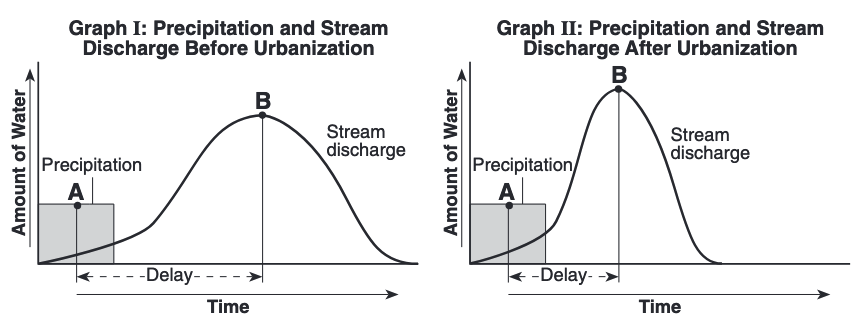
\includegraphics[width=5in]{hydrographs.png} 
   \caption{Hydrographs}
   \label{fig:hydrographs}
\end{figure}
\begin{enumerate}[a)]
\item What is a likely explaination for the delay time between points A and B?\\
~\\
~\\
~\\
~\\
\item How did urbanization affect delay time between points A and B?\\
~\\
~\\
~\\
~\\
\item How did urbanization affect the maximum stream discharge?\\
~\\
~\\
~\\
~\\
\end{enumerate}
\clearpage
%%%%%%%%%%%%%%%%%%%%%%%%%%%%%%%%%%%%%%%%%%%%%%%%%%%%
\item Figure \ref{fig:datatable} shows the average monthly discharge, in cubic feet per second, for a stream in New England.\newline

\begin{figure}[h!] %  figure placement: here, top, bottom, or page
   \centering
   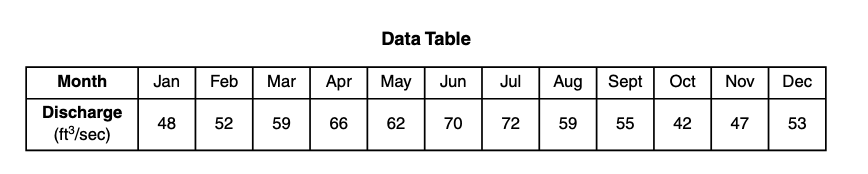
\includegraphics[width=5in]{datatable.png} 
   \caption{Tabular Data for New England Stream}
   \label{fig:datatable}
\end{figure}

\begin{enumerate}[a)]
\item On the grid on Figure \ref{fig:gridchart}, plot with an X the average stream discharge for
each month shown in the data table. \newline

\begin{figure}[h!] %  figure placement: here, top, bottom, or page
   \centering
   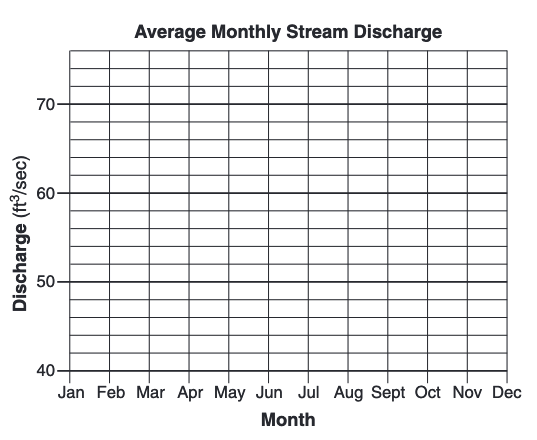
\includegraphics[width=5in]{gridchart.png} 
   \caption{Monthly Average Discharge for New England Stream}
   \label{fig:gridchart}
\end{figure}
\clearpage

\item Explain one possible reason why this stream’s discharge in April is greater than this stream’s discharge in January.\\
~\\
~\\
~\\
~\\
~\\
~\\
\item What is the average streamflow for this stream?\\
~\\
~\\
~\\
~\\
~\\
~\\
\item How many standard deviations from this average is the maximum monthly streamflow?\\
~\\
~\\
~\\
~\\
~\\
~\\
~\\
~\\
~\\
~\\
\item How many standard deviations from this average is the minimum monthly streamflow?\\
~\\
~\\
~\\
~\\
\end{enumerate}
\clearpage
\item Figure \ref{fig:watershed} is a small watershed comprised of two distinct land cover types.

\begin{figure}[h!] %  figure placement: here, top, bottom, or page
   \centering
   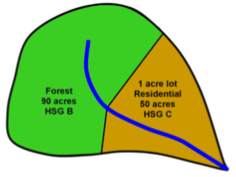
\includegraphics[width=3in]{watershed.png} 
   \caption{A watershed}
   \label{fig:watershed}
\end{figure}

The forest portion has a flow path length of 360 feet, at an average slope of 0.01 (1\%) until it reaches the residential portion whose path length is 430 feet, at an average slope of 0.005 (0.5\%). 

\begin{enumerate}[a)]
\item Determine the composite CN value for the watershed.\\
~\\
~\\
~\\
~\\
\item Estimate the time of concentration for the entire watershed using the NRCS-Upland method (Gupta pp. 718-720).\\
~\\
~\\
~\\
~\\
\end{enumerate}
\clearpage
\item A tabulation of an observed storm and associated runoff for the drainage area are listed below in Table \ref{tab:raro}. The runoff was measured at the culvert system and indicated by the blue circle on the map in Figure \ref{fig:culvert}.

\begin{figure}[h!] %  figure placement: here, top, bottom, or page
   \centering
   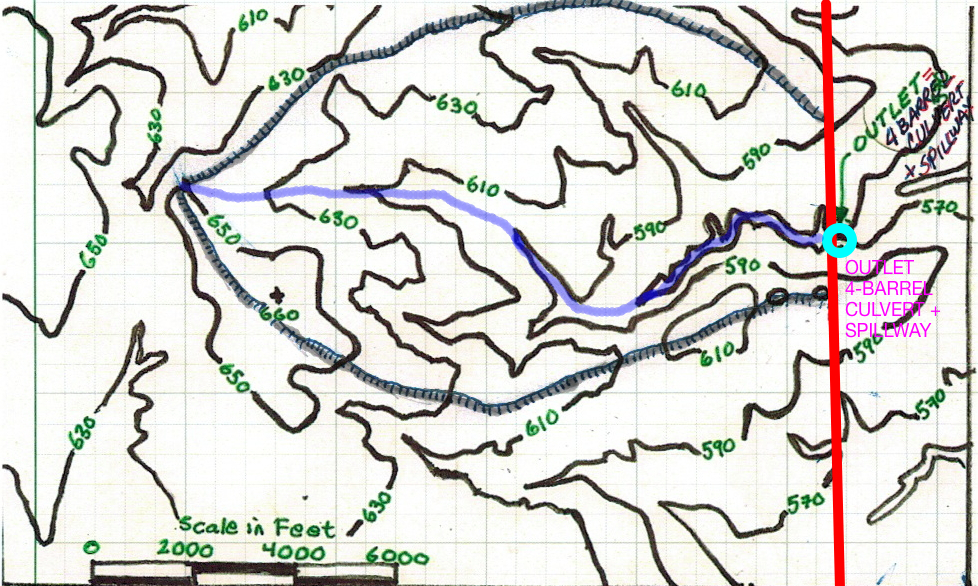
\includegraphics[width=6in]{topoMap.png} 
   \caption{Plan view of a small watershed draining to a culvert under a roadway}
   \label{fig:culvert}
\end{figure}


Determine

\begin{enumerate}[a)]
\item The approximate drainage area in $ft^2$ \clearpage
\item Complete Table \ref{tab:raro}


\begin{table}[h!]
\centering
\caption{Tabulated Rainfall and Runoff for Watershed}
\begin{tabular}{p{1.0in}p{1in}p{1in}p{1in}p{1in}} % Column formatting, @{} suppresses leading/trailing space
Time (hrs)&Accumulated Rain (inches)&Observed Discharge (cfs)&Incremental Volume (ft$^3$)&Cumulative Volume (ft$^3$)\\
\hline
\hline
0&0.000&0.00&~&~\\
1&0.000&0.00&~&~\\
2&0.000&0.00&~&~\\
3&0.000&0.00&~&~\\
4&0.000&0.00&~&~\\
5&0.000&0.00&~&~\\
6&0.000&0.00&~&~\\
7&0.000&0.00&~&~\\
8&0.101&0.20&~&~\\
9&0.106&0.31&~&~\\
10&0.111&0.31&~&~\\
11&0.115&0.31&~&~\\
12&0.120&0.31&~&~\\
13&0.120&0.40&~&~\\
14&0.150&0.40&~&~\\
15&0.750&24.66&~&~\\
16&2.750&588.23&~&~\\
17&2.940&808.70&~&~\\
18&3.030&154.28&~&~\\
19&3.030&94.68&~&~\\
20&3.030&27.56&~&~\\
21&3.090&36.13&~&~\\
22&3.210&19.65&~&~\\
23&3.300&7.00&~&~\\
24&3.300&0.00&~&~\\
\hline
\end{tabular}
\label{tab:raro}
\end{table}

\item The loss from the raw precipitation input to the watershed.\\
~\\
~\\
~\\
~\\
\clearpage
\item An appropriate CN for the watershed supported by the tabular data.\\
~\\
~\\
~\\
~\\
~\\
~\\
~\\
~\\
~\\
~\\
~\\
~\\
~\\
~\\
~\\
~\\
~\\
~\\
~\\
\item The maximum retention S for the watershed supported by the tabular data.\\
~\\
~\\
~\\
~\\
\end{enumerate}

\clearpage
%%%%%%%%%%%%%%%%%%%%%%%%%%%%%%%%%%%%%%%%%%%%%%%%%%%%%%%%%%%%%

\item Figure \ref{fig:UnitHydrographInput} is the unit hydrograph response for a watershed to a 1-hour long \textbf{excess rainfall} event of intensity equal to 1-inch/hour.  

\begin{figure}[htbp] %  figure placement: here, top, bottom, or page
   \centering
   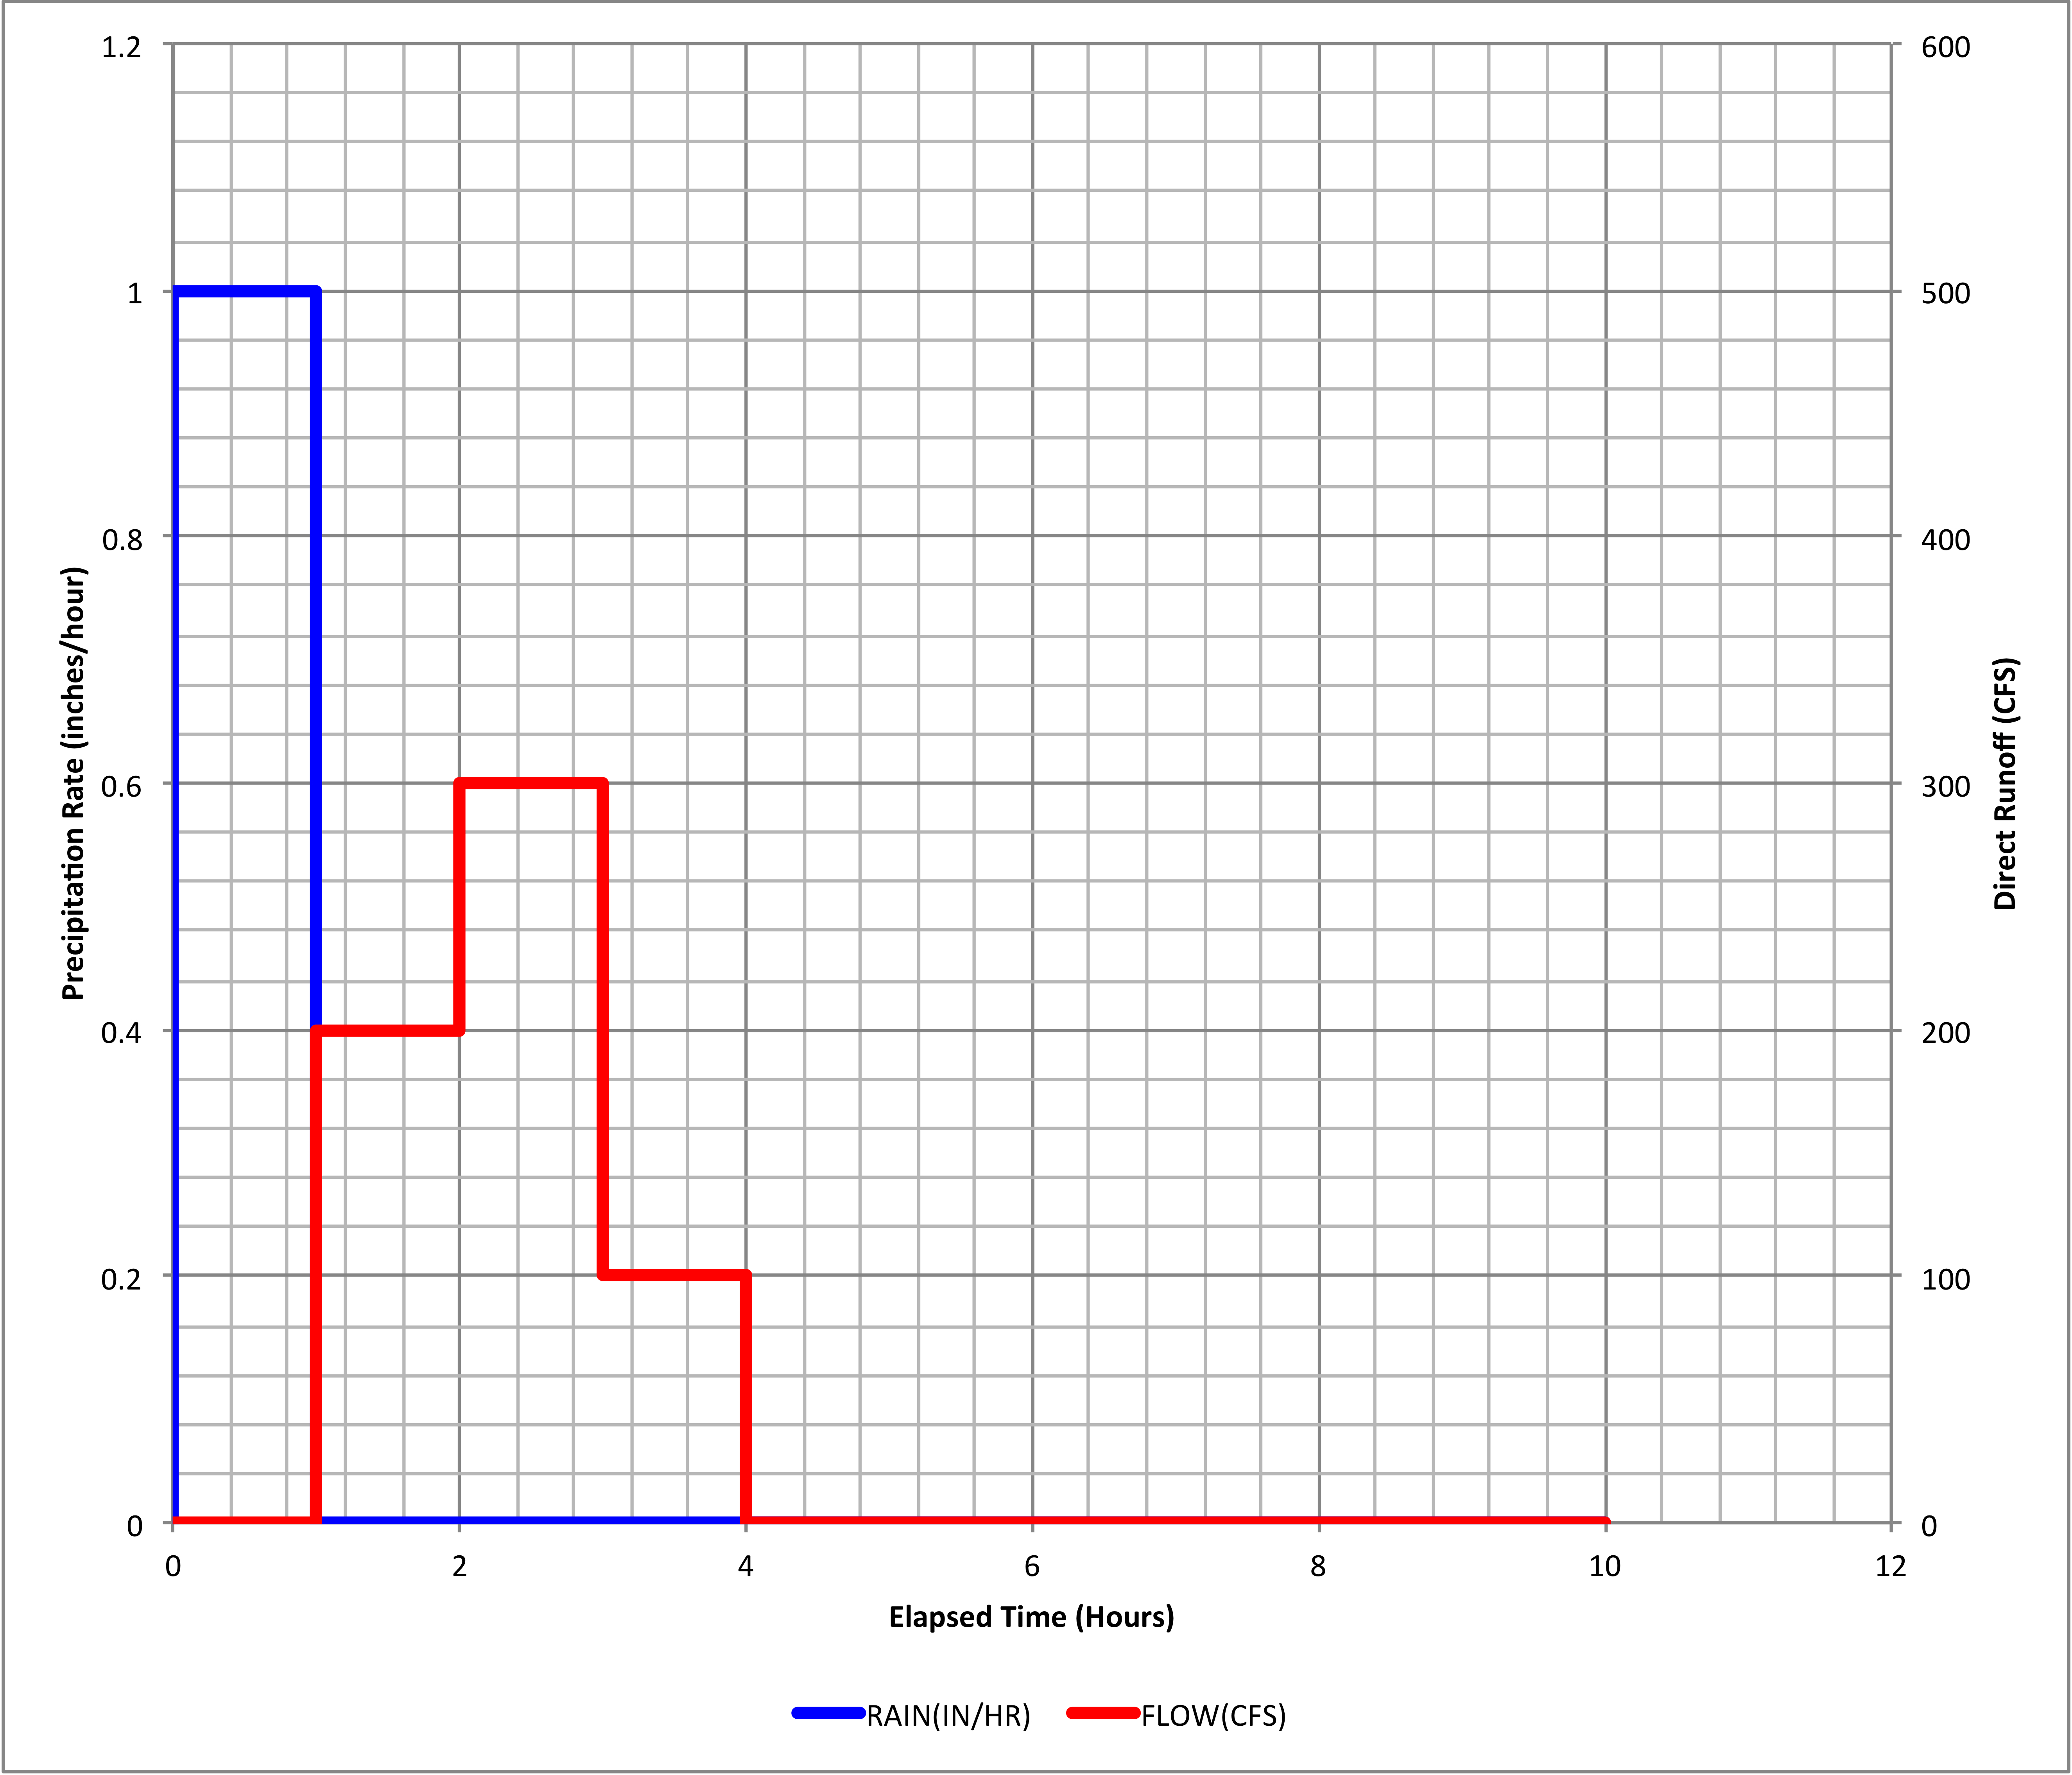
\includegraphics[width=5in]{UnitHydrographInput.png} 
   \caption{Unit hydrograph response (red) to a 1-inch per hour constant intensity precipitation (blue) input.}
   \label{fig:UnitHydrographInput}
\end{figure}

\begin{enumerate}[a)]
\item What is the meaning of \textbf{excess rainfall}?\\
~\\
~\\
~\\
~\\
\item How many non-zero intervals of (including the hour zero to hour one interval) direct runoff are indicated by the unit hydrograph? \\
\clearpage
\item What is the maximum discharge in CFS indicated by the unit hydrograph?\\
~\\
~\\
\item What is the total volume (in $ft^3$) of runoff depicted by the unit hydrograph? \\
~\\
~\\
~\\
~\\
~\\
~\\
~\\
~\\
~\\
~\\
~\\
~\\
~\\
~\\
\item Compute the watershed area (in $mi^2$) of the watershed? \\
\clearpage
\begin{figure}[htbp] %  figure placement: here, top, bottom, or page
   \centering
   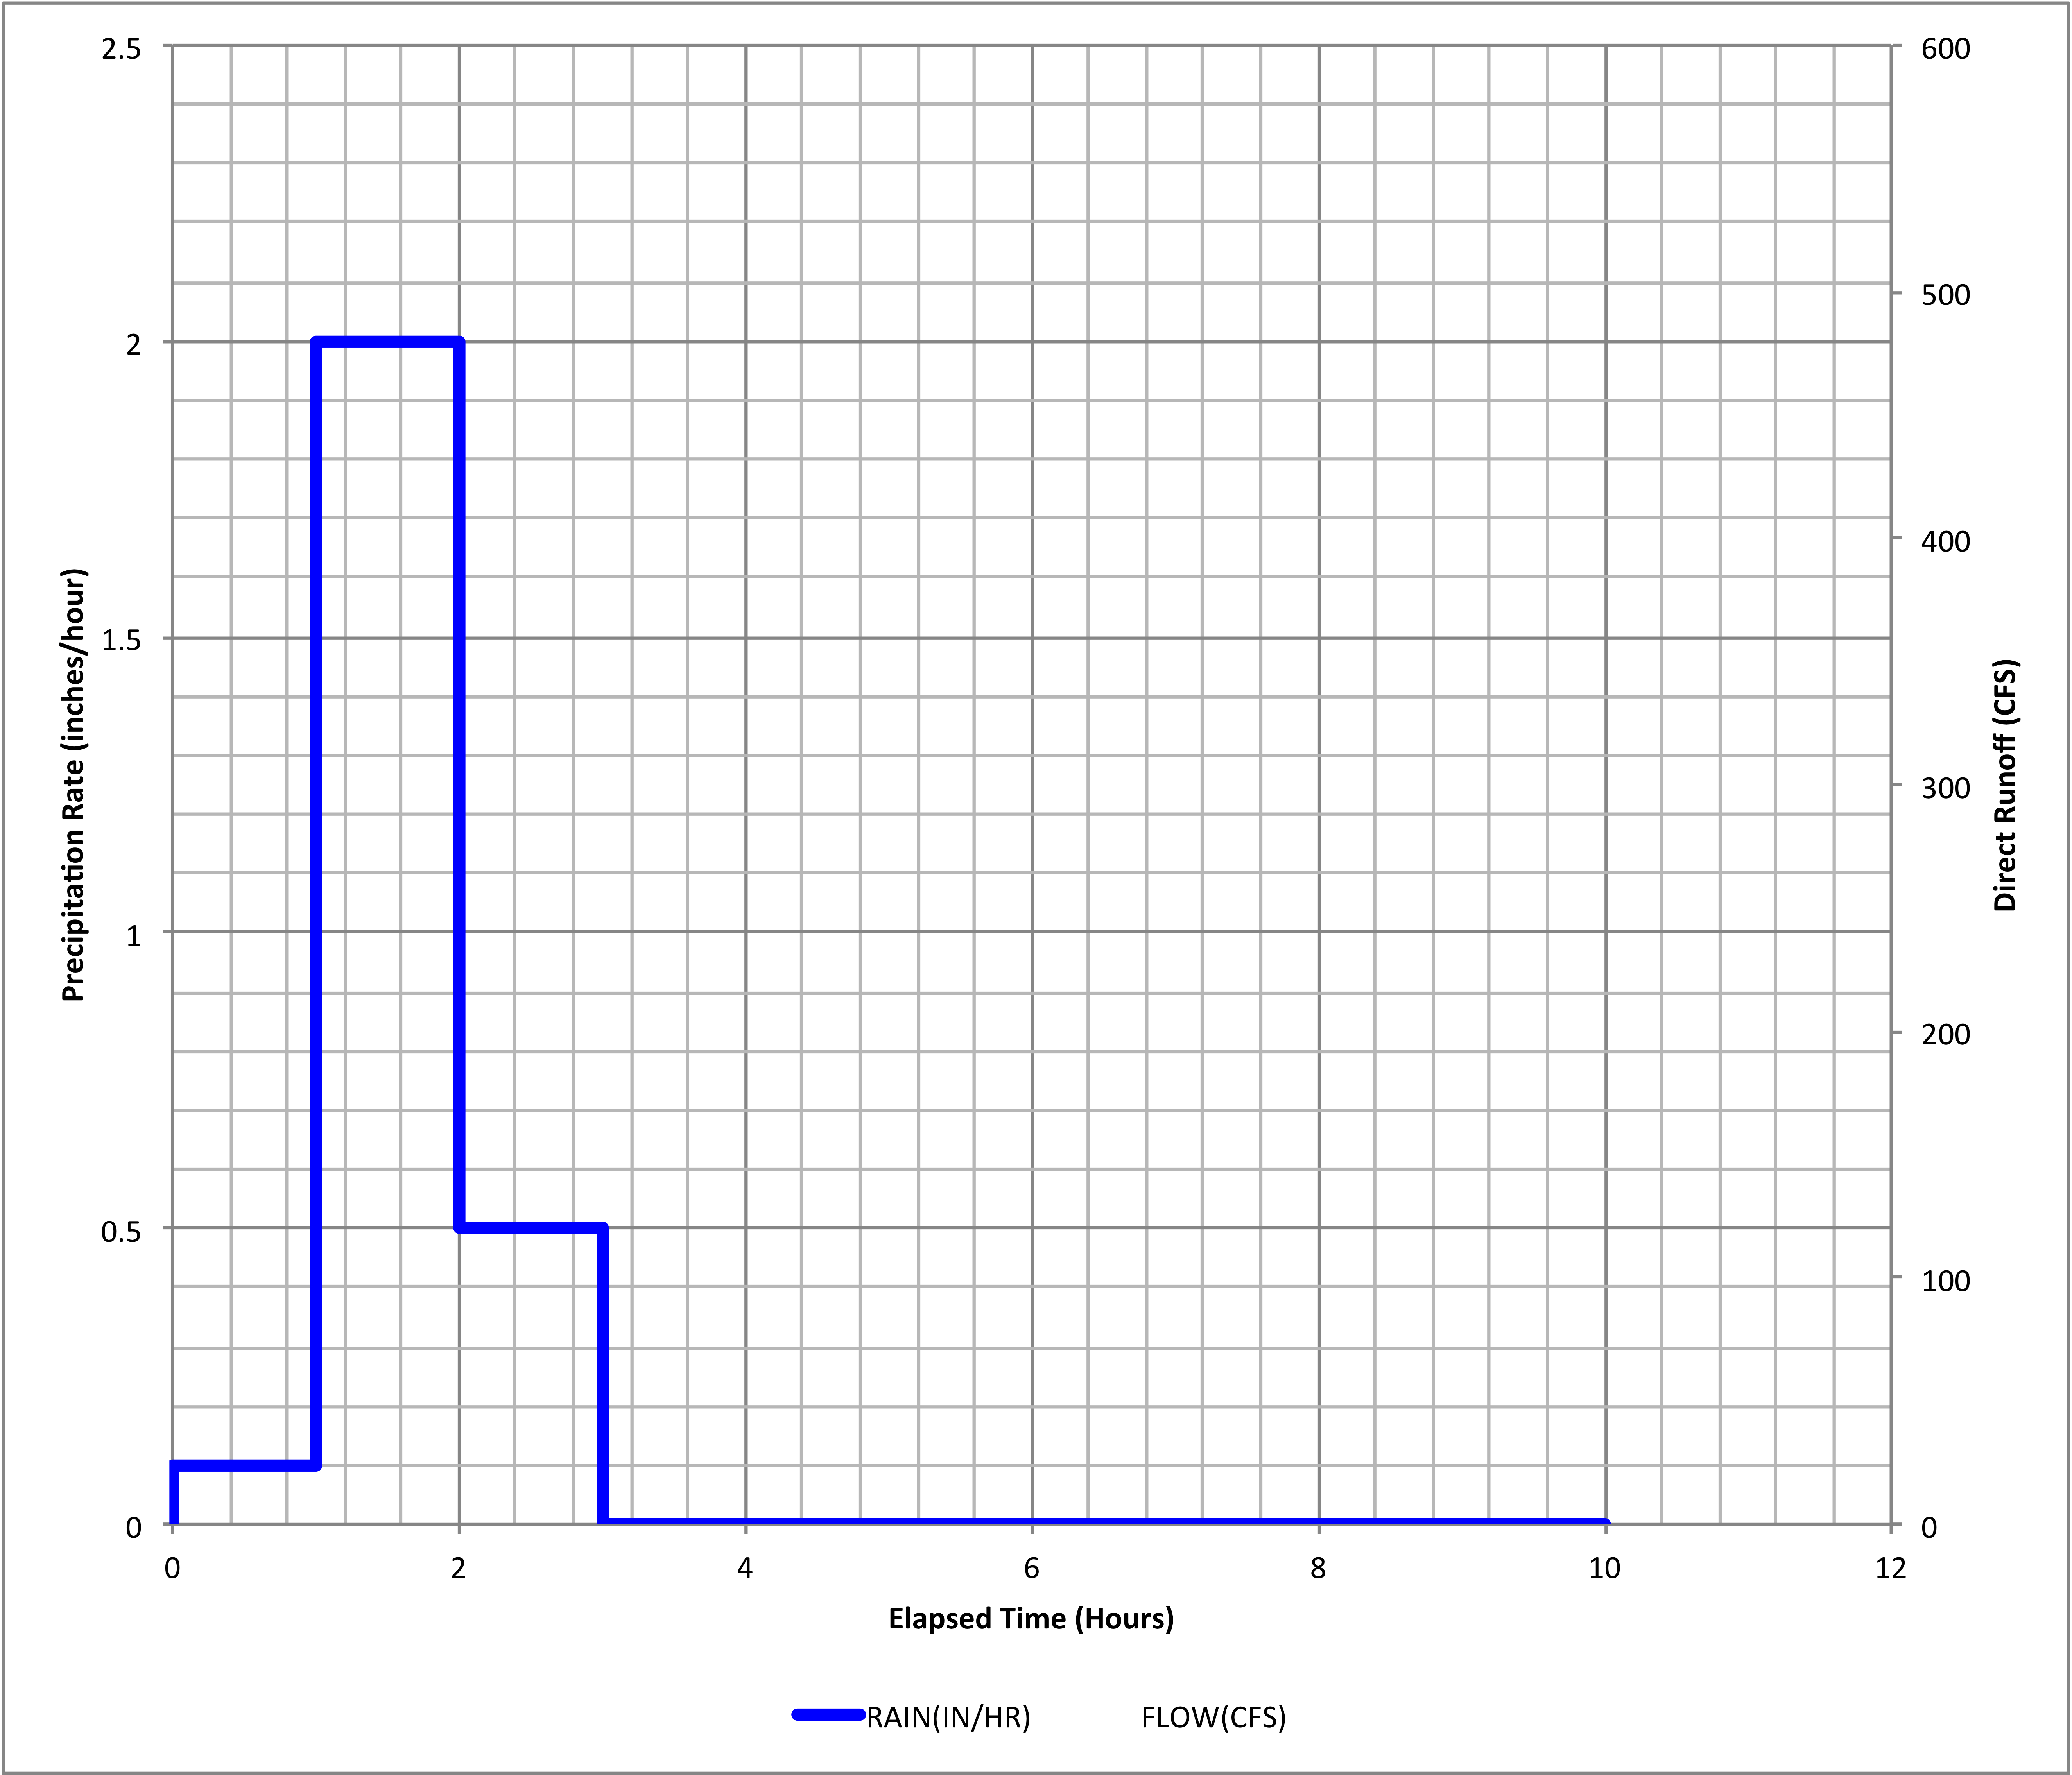
\includegraphics[width=5in]{UnitHydrographOutput.png} 
   \caption{3-hour event comprised of 3 consecutive 1-hour events.}
   \label{fig:UnitHydrographOutput}
\end{figure}
\item What is the total volume (in $ft^3$) of runoff anticipated for the storm depicted in Figure \ref{fig:UnitHydrographOutput}?  \\
~\\
~\\
~\\
~\\
\item Plot the response to the 3 consecutive 1-hour events with the intensities indicated in Figure \ref{fig:UnitHydrographOutput}.
\end{enumerate}



\clearpage
%%%%%%%%%%%%%%%%%%%%%%%%%%%

\item What is a synthetic unit hydrograph?
\begin{enumerate}[a)]
\item A unit hydrograph derived directly from observed rainfall-runoff data.
\item A unit hydrograph estimated using empirical equations and watershed characteristics.
\item A hydrograph that measures both rainfall and runoff over a synthetic watershed.
\item A hydrograph that uses only temperature and humidity data to predict runoff.
\end{enumerate}

\item Which of the following parameters is typically used to construct a synthetic unit hydrograph?
\begin{enumerate}[a)]
\item Soil moisture and groundwater levels.
\item Watershed area, time of concentration, and peak discharge.
\item Evaporation rates and relative humidity.
\item Daily rainfall totals for the region.
\end{enumerate}

\item Which synthetic unit hydrograph method is widely used in the United States for small and medium-sized watersheds?
\begin{enumerate}[a)]
\item Rational Method.
\item Horton Method.
\item Soil Conservation Service (SCS) Method.
\item Kinematic Wave Method.
\end{enumerate}

\item In Snyder's Synthetic Unit Hydrograph method, which factor represents the lag time between the centroid of rainfall and the peak of the hydrograph?
\begin{enumerate}[a)]
\item Time of concentration.
\item Basin lag coefficient.
\item Peak discharge coefficient.
\item Runoff coefficient.
\end{enumerate}
\clearpage
%%%%%%%%%%%%%%%%%%%%%%%%%%
\item What is one advantage of using a synthetic unit hydrograph over an observed unit hydrograph?
\begin{enumerate}[a)]
\item It requires extensive streamflow data from multiple storm events.
\item It can be applied to ungauged watersheds where no direct runoff data is available.
\item It eliminates the need for watershed parameterization.
\item It provides a more accurate prediction of runoff for every storm event.
\end{enumerate}

\clearpage
%%%%%%%%%%%%%
\end{enumerate}
\end{document}
